% Provenance (never printed): see sources/outline_sources.md (Year 1: morphology,
% gravity, heat flow and seismicity of a subduction zone; accretionary and erosive
% margins; slab geometry; volcanic arcs). Kuril map, section and numbers from
% figdata/bachelor-1/slab_seismicity.py; exercise and problem values in the Book 3
% scratch calculator calc/ch14.py.
\chapter{活动大陆边缘}\label{ch:b1:active-margins}

2011 年 3 月 11 日当地时间 14:46，日本东北部外海的板块边界
沿\omterm{def:b1:active-margins:active-margin}{海沟}破裂约 \qty{400}{km}，沿\omterm{def:b1:geological-maps:attitude}{倾向}向下延伸 \qty{150}{km}。
断层滑移量达 50 至 \qty{60}{m}，大部分位于
震源上倾方向、朝向日本\omterm{def:b1:active-margins:active-margin}{海沟}；陆上海岸水平移动并
沉降。此处下沉的板块为太平洋板块，俯冲于
日本之下，沿一个由地震勾勒出的面向下延伸数百千米；
当该面位于约一百千米深处时，一列火山
平行于海岸延伸。本章由其形态、
重力、\omterm{def:b1:heat-budget:heat-flow}{热流}，尤其是地震活动，来解读此类边缘。
% ledger: usgs:tohoku, wada:decoupling

\begin{recall}
大洋\omterm{def:b1:layered-earth:lithosphere}{岩石圈}在俯冲带处重新沉入\omterm{def:b1:layered-earth:layers}{地幔}，俯冲带以
\omterm{def:b1:active-margins:active-margin}{海沟}和倾斜的地震带为标志，古老\omterm{def:b1:layered-earth:lithosphere}{岩石圈}在
自身重力作用下沉（第 2 册，十一年级）；下沉板块释出的水降低了
其上方\omterm{def:b1:layered-earth:layers}{地幔}的熔化温度（第 2 册，十二年级）。热量
扩散距离 $L$ 所需时间量级为 $L^2/\kappa$（见\cref{ch:b1:heat-budget}）；
无限大板片（密度 $\rho$、厚度 $h$）的吸引力为 $2\pi G\rho h$
（见\cref{ch:b1:isostasy-gravity}）；板块绕\omterm{def:b1:plate-kinematics:euler-pole}{欧拉极}运动；
（见\cref{ch:b1:plate-kinematics}）；洋底\omterm{def:b1:heat-budget:heat-flow}{热流}随
其年龄的平方根倒数而减小（见\cref{ch:b1:rifts-ridges-margins}）。
\end{recall}

\section{活动大陆边缘的结构}\label{sec:b1:active-margins:anatomy}

\begin{definition}[活动大陆边缘、海沟、弧前、弧后盆地]\label{def:b1:active-margins:active-margin}
称\emph{活动大陆边缘}\index{活动大陆边缘}为汇聚型板块边界，在该边界
处大洋\omterm{def:b1:layered-earth:lithosphere}{岩石圈}俯冲于另一板块之下，既可俯冲于大陆之下，
也可俯冲于另一大洋板块之下。\emph{海
沟}\index{海沟}是海底狭长、呈 V 形的凹陷，
下沉板块沿此凹陷弯曲并俯冲于另一板块之下。
\emph{弧前}\index{弧前}是上覆板块位于
海沟与\omterm{def:b1:active-margins:volcanic-arc}{火山弧}之间的部分。\emph{弧后盆地}\index{弧后盆地}
是位于\omterm{def:b1:active-margins:volcanic-arc}{火山弧}后方、远离海沟一侧的盆地，
该处上覆板块受拉伸，可能形成新的\omterm{def:b1:rifts-ridges-margins:oceanic-crust}{洋壳}。
\end{definition}

\omterm{def:b1:active-margins:active-margin}{海沟}是大洋中最深的地方，其中最深者为
马里亚纳\omterm{def:b1:active-margins:active-margin}{海沟}中的挑战者深渊。穿越千岛\omterm{def:b1:active-margins:active-margin}{海沟}时，海底
由深海平原上约 \qty{5200}{m} 降至\omterm{def:b1:active-margins:active-margin}{海沟}轴部的 \qty{8700}{m}，
低约 \qty{3.5}{km}，\omterm{def:b1:active-margins:active-margin}{海沟}宽度仅数十千米
（图见\cref{sec:b1:active-margins:gravity-heat}）。地球上的汇聚型边缘
总长约 \qty{55000}{km}；在板块边界的数字模型中，
俯冲型边界合计约 \qty{51000}{km}，
而扩张洋脊约 \qty{67000}{km}。
% ledger: data:b3-grav-kuril (trench_gravity.py values), stern:subduction, data:pb2002 (ridge_budget.py)

在\omterm{def:b1:active-margins:active-margin}{海沟}海侧，板块在俯冲前略有隆起，形成一个宽阔的
低矮的外隆起。该处板块发生弯曲，其上部受拉伸：
正断层型地震发生于外隆起处。外隆起的宽度
与弹性板块的弯曲相符；\omterm{def:b1:layered-earth:lithosphere}{岩石圈}的这种挠曲
在第 5 册中研究。\omterm{def:b1:active-margins:active-margin}{海沟}即是致密下沉板块的
重量将其前缘向下拉拽之处。

\begin{definition}[俯冲板片]\label{def:b1:active-margins:slab}
称\emph{俯冲板片}\index{俯冲板片}为下沉板块中
已经进入\omterm{def:b1:layered-earth:layers}{地幔}的部分：一块大洋\omterm{def:b1:layered-earth:lithosphere}{岩石圈}
薄板，\omterm{def:b1:rifts-ridges-margins:oceanic-crust}{洋壳}位于其上部，自\omterm{def:b1:active-margins:active-margin}{海沟}起倾斜伸入上覆板块之下，
直至数百千米深处。
\end{definition}

上覆板块被沿平行于\omterm{def:b1:active-margins:active-margin}{海沟}的方向切分为若干条带
（见下图）：\omterm{def:b1:active-margins:active-margin}{弧前}，其前缘常堆积着
被刮落的沉积物，其后为沉积盆地；
\omterm{def:b1:active-margins:volcanic-arc}{火山弧}；在部分\omterm{def:b1:active-margins:volcanic-arc}{火山弧}后方还有\omterm{def:b1:active-margins:active-margin}{弧后盆地}，其外侧
为一条更古老、已灭绝的\omterm{def:b1:active-margins:volcanic-arc}{火山弧}。板片与上覆板块之间
夹有一楔\omterm{def:b1:layered-earth:layers}{地幔}，沿板片顶部被拖曳下行。

\begin{omfigure}
\begin{tikzpicture}[x=0.01667cm, y=0.01667cm, font=\scriptsize,
  lbl/.style={fill=white, fill opacity=0.8, text opacity=1, inner sep=1pt}]
\begin{scope}
\clip (-150,-330) rectangle (650,55);
% mantle and sea water
\fill[orange!12] (-150,-330) rectangle (650,15);
\fill[omSea!45] (-150,15) rectangle (650,0);
% incoming plate and slab: top dips 25 deg to 50 km, then 45 deg; 100 km thick
\fill[omLithBasalt!55] (-150,4) -- (-80,4) .. controls (-60,7) and (-40,7) .. (-25,4) -- (0,0)
  -- (107.2,-50) -- (420,-363) -- (349,-434) -- (48.9,-133.1) -- (-22.1,-100) -- (-150,-100) -- cycle;
\draw[omSea!50!black, line width=1.6pt] (-150,4) -- (-80,4) .. controls (-60,7) and (-40,7) .. (-25,4) -- (0,0) -- (107.2,-50) -- (420,-363);
% overriding plate
\fill[brown!28] (0,0) -- (12,3) -- (45,8) -- (60,10) -- (140,10) -- (150,12) -- (184,12) -- (230,9)
  -- (300,7) -- (395,6) -- (410,3) -- (420,2) -- (430,3) -- (445,6) -- (540,7) -- (560,14) -- (590,14)
  -- (610,10) -- (650,10) -- (650,-60) -- (520,-55) -- (445,-25) -- (420,-15) -- (395,-25) -- (320,-55)
  -- (250,-60) -- (117.2,-60) -- (107.2,-50) -- cycle;
% accretionary prism and forearc basin
\fill[yellow!55] (0,0) -- (12,3) -- (45,8) -- (60,10) -- (60,-28) -- cycle;
\draw[black!45, line width=0.3pt] (14,-3) -- (24,5) (28,-7) -- (38,6) (42,-14) -- (52,8);
\fill[yellow!30] (68,10) -- (132,10) -- (122,4) -- (78,4) -- cycle;
% arc volcano
\fill[black!60] (150,12) -- (167,26) -- (184,12) -- cycle;
% an isotherm: a cold tongue down the slab
\draw[omDef, dashed, line width=0.6pt] (-150,-82) -- (-30,-82) -- (40,-118) -- (300,-318)
  -- (232,-200) -- (150,-112) .. controls (130,-80) and (180,-72) .. (260,-72) -- (650,-72);
% mantle wedge flow
\draw[->, black!60, line width=0.5pt] (600,-130) .. controls (450,-135) and (300,-125) .. (215,-150)
  .. controls (205,-160) and (240,-185) .. (300,-235);
% water and melt
\foreach \x/\z in {150/-93, 172/-115, 194/-137}
  \draw[->, blue!70!black, line width=0.5pt] (\x,\z) -- (\x-6,\z+28);
\draw[red!75!black, line width=0.8pt, decorate, decoration={snake, amplitude=1.2, segment length=6}] (167,-100) -- (167,12);
% earthquakes
\foreach \x/\z in {20/-12, 45/-22, 70/-34, 95/-45, 60/-40, 85/-58, 120/-70, 135/-85, 150/-104,
  165/-112, 185/-140, 205/-150, 225/-175, 248/-195, 270/-216, 290/-242, 312/-262, 330/-282, 350/-300, 365/-318}
  \fill[black] (\x,\z) circle[radius=0.9pt];
% the 100-km level beneath the arc
\draw[black!70, densely dotted] (90,-100) -- (260,-100);
\draw[black!70, densely dotted] (167,12) -- (167,-110);
\end{scope}
\draw[black!70] (-150,-330) rectangle (650,55);
\node[lbl, anchor=south] at (-85,15) {外隆起};
\node[lbl, anchor=south] at (0,15) {海沟};
\node[lbl, anchor=west] (pr) at (75,-28) {增生楔};
\draw[black!70] (pr.west) -- (38,-6);
\node[lbl, anchor=south] at (88,15) {弧前};
\node[lbl, anchor=south] at (185,27) {火山弧};
\node[lbl, anchor=south] at (420,15) {弧后盆地};
\node[lbl, anchor=south] at (575,15) {残留弧};
\node[lbl, anchor=west] at (-140,-50) {大洋岩石圈};
\node[lbl, anchor=east] (sl) at (120,-262) {俯冲板片};
\draw[black!70] (sl.east) -- (205,-262);
\node[lbl, anchor=west] (wb) at (420,-265) {和达–贝尼奥夫带};
\draw[black!70] (wb.west) -- (318,-266);
\node[lbl] at (430,-170) {地幔楔};
\node[lbl] at (575,-30) {上覆板块};
\node[lbl, anchor=west, text=blue!70!black] at (212,-98) {水};
\node[lbl, anchor=east] at (88,-100) {深 \qty{100}{km}};
\node[lbl, anchor=west, text=omDef] at (450,-95) {等温线};
\node[lbl, anchor=west] at (-140,-300) {地幔};
\draw[line width=1pt] (500,-310) -- (600,-310) node[midway, above] {\qty{100}{km}};
\end{tikzpicture}
\par\smallskip{\small 俯冲带剖面（示意图：\omterm{def:b1:layered-earth:lithosphere}{岩石圈}与板片
依线段比例尺绘制，海底以上地形被大幅夸大）。
板片在\omterm{def:b1:active-margins:active-margin}{弧前}之下\omterm{def:b1:geological-maps:attitude}{倾角}较缓，再向深处更陡；\omterm{def:b1:active-margins:volcanic-arc}{火山
弧}位于板片顶面约 \qty{100}{km}
深处的正上方。冷板片将其等温线拖入\omterm{def:b1:layered-earth:layers}{地幔}（虚线：一条
等温线），\omterm{def:b1:layered-earth:layers}{地幔}楔亦沿其被拖拽下沉。圆点表示
地震，分布于靠近\omterm{def:b1:active-margins:active-margin}{海沟}的板块边界以及下方板片内部。
板片释放的水上升进入\omterm{def:b1:layered-earth:layers}{地幔}楔；熔体上升至\omterm{def:b1:active-margins:volcanic-arc}{火山弧}。}
\label{fig:b1:active-margins:section}
\end{omfigure}

在同一数字模型上求和，每年约有 \qty{2.7}{km^2} 的洋底
沿俯冲边界沉没，接近洋中脊生成的 \qty{3.0}{km^2}
（见\cref{ch:b1:rifts-ridges-margins}）。在这类模型的精度之内，该模型略去了宽阔板块边界带的缓慢变形，
洋底被消亡的速度与其生成速度大致相当，
地球表面
的面积因此保持不变。
% ledger: data:pb2002 (ridge_budget.py: consumed 2.74, made 3.01 km2/yr)

\section{重力与热流}\label{sec:b1:active-margins:gravity-heat}

费利克斯·韦宁·梅内斯发现了沿\omterm{def:b1:active-margins:active-margin}{海沟}分布的长而窄的负\omterm{def:b1:isostasy-gravity:anomalies}{重力异常}带
（见\cref{ch:b1:isostasy-gravity}）。如今卫星可以在海上处处测绘这些异常。
横穿千岛\omterm{def:b1:active-margins:active-margin}{海沟}（见下图），\omterm{def:b1:isostasy-gravity:anomalies}{自由空气异常}在外隆起上方升至约
\qty{40}{\milli\gal}，在\omterm{def:b1:active-margins:active-margin}{海沟}上方降至
\qty{-260}{\milli\gal}，随后在\omterm{def:b1:active-margins:active-margin}{弧前}
与\omterm{def:b1:active-margins:volcanic-arc}{火山弧}的岛屿上方再次强烈为正。
% ledger: egs:vening-meinesz, data:b3-grav-kuril (trench_gravity.py values: rise 38 mGal at -155 km, low -260 at 0, high 218 at 160 km)

\omterm{def:b1:active-margins:active-margin}{海沟}异常的大小说明\omterm{def:b1:active-margins:active-margin}{海沟}是如何被支撑的。假设\omterm{def:b1:active-margins:active-margin}{海沟}
比周围海底深 \qty{3.5}{km}，且完全未得到补偿：
那么在\omterm{def:b1:active-margins:active-margin}{海沟}处，\qty{3.5}{km} 厚、密度约为
\qty{2700}{kg.m^{-3}} 的岩石将被海水取代。由布格板
（见\cref{prop:b1:isostasy-gravity:slab}）可知，那里的重力将偏低
\[
  2\pi G\,\Delta\rho\,h = 2\pi \times \num{6.674e-11} \times 1700 \times 3500
  \approx \qty{2.5e-3}{m.s^{-2}} = \qty{250}{\milli\gal} .
\]
这正是观测到的低值。因此\omterm{def:b1:active-margins:active-margin}{海沟}并不处于
\omterm{def:b1:isostasy-gravity:isostasy}{地壳均衡}状态：它是一个被压低的凹陷，由弯曲板块的强度与板片拉力
维持，抗衡其下方\omterm{def:b1:layered-earth:layers}{地幔}的浮力。（
仅几十千米宽的\omterm{def:b1:active-margins:active-margin}{海沟}，其吸引作用小于无限大板片，因此
仅其中的海水产生的异常略小于此值；亏损的其余部分
位于更深处，那里整个弯曲的板块（包括其较轻的\omterm{def:b1:layered-earth:layers}{地壳}）被压入
\omterm{def:b1:layered-earth:layers}{地幔}之中，参见练习~\ref{exo:b1:active-margins:1}）。

\begin{omfigure}
\begin{tikzpicture}
\begin{axis}[omrecord, name=grav, width=0.86\linewidth, height=4.6cm, xmin=-250, xmax=450,
  ymin=-300, ymax=260, ylabel={自由空气 (\unit{\milli\gal})}, ylabel style={at={(-0.075,0.5)}}, xticklabels={},
  ytick={-200,-100,0,100,200}, clip=false]
% computed in figdata/bachelor-1/trench_gravity.py; ledger: data:b3-grav-kuril
\addplot[black!30, forget plot] coordinates {(-250,0) (450,0)};
\addplot[omDef, line width=1pt] table[x=x, y=faa] {figdata/out/bachelor-1-trench_gravity-profile.dat};
\draw[black!50, densely dotted] (axis cs:0,-300) -- (axis cs:0,260) (axis cs:164,-300) -- (axis cs:164,260);
\node[font=\scriptsize, anchor=south] at (axis cs:-155,45) {外隆起，$+38$};
\node[font=\scriptsize, anchor=west] at (axis cs:12,-262) {海沟，$-260$};
\node[font=\scriptsize, anchor=south west] at (axis cs:200,140) {弧前及火山弧};
\end{axis}
\begin{axis}[omrecord, at={(grav.south)}, anchor=north, yshift=-0.45cm, width=0.86\linewidth, height=4.6cm,
  xmin=-250, xmax=450, ymin=20, ymax=100, ylabel={热流 (\unit{mW.m^{-2}})}, ylabel style={at={(-0.075,0.5)}},
  xlabel={距海沟距离，朝向上覆板块方向 (\unit{km})}, clip=false]
% schematic; levels from the ledger: parsons:plate-model (11.3/sqrt(122) x 41.84 = 42.8 mW/m2 for the
% 122-Myr Kuril plate), hyndman:backarc (70-85); the forearc low is drawn without a value (wada:decoupling)
\addplot[fill=omDef!15, draw=none, forget plot] coordinates {(190,70) (450,70) (450,85) (190,85)} -- cycle;
\addplot[omProp!80!black, line width=1pt, smooth, tension=0.5] coordinates {(-250,43) (-60,43) (-10,41) (30,36) (120,36)
  (150,48) (180,76) (230,78) (450,78)};
\draw[black!50, densely dotted] (axis cs:0,20) -- (axis cs:0,100) (axis cs:164,20) -- (axis cs:164,100);
\node[font=\scriptsize, anchor=south] at (axis cs:-130,44) {老洋底，约 43};
\node[font=\scriptsize, anchor=north] at (axis cs:75,34) {弧前：偏低};
\node[font=\scriptsize, anchor=south] at (axis cs:320,85) {火山弧与弧后，70 至 85};
\node[font=\scriptsize, anchor=north west] at (axis cs:3,99) {海沟};
\node[font=\scriptsize, anchor=north west] at (axis cs:167,99) {火山弧};
\end{axis}
\end{tikzpicture}
\par\smallskip{\small 俯冲带两侧的重力与\omterm{def:b1:heat-budget:heat-flow}{热流}。上图：
卫星测得的横穿千岛\omterm{def:b1:active-margins:active-margin}{海沟}的自由空气\omterm{def:b1:isostasy-gravity:anomalies}{重力异常}，沿
\cref{sec:b1:active-margins:seismicity}中图示的剖面：
外隆起上方 \qty{38}{\milli\gal}，\omterm{def:b1:active-margins:active-margin}{海沟}上方 \qty{-260}{\milli\gal}，
\omterm{def:b1:active-margins:active-margin}{弧前}及岛屿上方强烈为正。下图：\omterm{def:b1:heat-budget:heat-flow}{热流}，
为示意剖面：老洋底上约 \qty{43}{mW.m^{-2}}，
\omterm{def:b1:active-margins:active-margin}{弧前}处较低，\omterm{def:b1:active-margins:volcanic-arc}{火山弧}与弧后上方平均为 70 至 \qty{85}{mW.m^{-2}}，
虚线：\omterm{def:b1:active-margins:active-margin}{海沟}与火山前缘。数据：Scripps
Institution of Oceanography 海洋重力模型（Sandwell 等，2014）。}
\label{fig:b1:active-margins:profiles}
\end{omfigure}

\omterm{def:b1:heat-budget:heat-flow}{热流}从另一侧印证了同样的结论。老洋底
进入\omterm{def:b1:active-margins:active-margin}{海沟}时损失的热量很少，约为 \qty{43}{mW.m^{-2}}，
这是按\cref{ch:b1:rifts-ridges-margins}的规律对千岛板块（\qty{122}{Ma}）算得的值。
\omterm{def:b1:active-margins:active-margin}{弧前}上方的\omterm{def:b1:heat-budget:heat-flow}{热流}更低：其下的冷板片从上方吸收
热量，\omterm{def:b1:active-margins:active-margin}{弧前}之下的\omterm{def:b1:layered-earth:layers}{地幔}寒冷而停滞。在\omterm{def:b1:active-margins:volcanic-arc}{火山弧}
与弧后，\omterm{def:b1:heat-budget:heat-flow}{热流}较高，平均为 70 至 \qty{85}{mW.m^{-2}}，约为
老大陆内部\omterm{def:b1:heat-budget:heat-flow}{热流}（约 \qty{40}{mW.m^{-2}}）的两倍。活动
\omterm{def:b1:active-margins:volcanic-arc}{火山弧}需要\omterm{def:b1:layered-earth:layers}{地幔}楔处于约 \qty{1200}{\celsius}，
位于地下约 \qty{100}{km} 处；其后的整个弧后都很热，\omterm{def:b1:layered-earth:lithosphere}{岩石圈}
厚度仅 50 至 \qty{60}{km}，\omterm{def:b1:layered-earth:discontinuity}{莫霍面}温度达 800 至 \qty{900}{\celsius}。
% ledger: parsons:plate-model (11.3/sqrt(122) x 41.84 = 42.8), wada:decoupling, hyndman:backarc

板片为何保持低温？因为它下沉的速度快于其升温的速度。
\cref{sec:b1:active-margins:seismicity}中的千岛板片以约
\qty{82}{mm} 的速度俯冲，\omterm{def:b1:geological-maps:attitude}{倾角} \ang{45}：到达 \qty{600}{km} 深处需经过
长 $600/\sin\ang{45} \approx \qty{850}{km}$ 的路径，约需一千万年。
由热传导时间尺度（见\cref{prop:b1:heat-budget:timescale}）可知，来自
\omterm{def:b1:layered-earth:layers}{地幔}的热量穿过 \qty{50}{km} 到达 \qty{100}{km} 厚板片的中部，所需时间为
\[
  \tau = \frac{L^2}{\kappa} = \frac{(\qty{5e4}{m})^2}{\qty{e-6}{m^2.s^{-1}}}
  = \qty{2.5e15}{s} \approx \qty{80}{Ma},
\]
约长八倍。板片的核心抵达 \qty{600}{km} 深处时，几乎
与其在\omterm{def:b1:active-margins:active-margin}{海沟}处时一样寒冷，等温线随之被拖入深处，
如上图俯冲带剖面所示。
% values (slab_seismicity.py): vel_normal 81.66 mm/yr, dip 44.9; calc/ch14.py

\section{地震与板片的形状}\label{sec:b1:active-margins:seismicity}

\begin{definition}[和达–贝尼奥夫带]\label{def:b1:active-margins:wadati-benioff}
称\emph{和达–贝尼奥夫带}\index{和达–贝尼奥夫带}为一条倾斜的地震带，
由地震构成，始于\omterm{def:b1:active-margins:active-margin}{海沟}附近，并在上覆板块之下逐渐加深，
深度可达约 \qty{700}{km}，它勾勒出\omterm{def:b1:active-margins:slab}{俯冲板片}的轮廓。
\end{definition}
% ledger: usgs:deepest

它的地震分两类。深至几十千米处，地震发生在
板块边界本身，即两板块相互错动滑过的缓倾断层上；
地球上最大的地震，例如 2011 年日本近海的那次，
正是沿这条断层破裂的。更深处，地震发生在板片内部，
唯有板片仍足够冷，能够积累应力。在最大深度处，板片甚至应当
发生流动而非破裂，地震究竟从何深度开始，至今仍有争议。
目录中最深的地震，震级为 4.2，发生于
2004 年瓦努阿图地区之下 \qty{735.8}{km} 处。在所考察的每一个俯冲带中，
这些俯冲带在中等深度处呈双层结构：两层地震，
板块越老，两层相距越远。
% ledger: usgs:deepest, brudzinski:double, usgs:tohoku

千岛群岛位于北海道与堪察加之间，其下为一块板片，地震
勾勒出自\omterm{def:b1:active-margins:active-margin}{海沟}向下直至 \qty{600}{km} 以上的轮廓。此处太平洋板块抵达\omterm{def:b1:active-margins:active-margin}{海沟}时，年龄约为 1.2 亿年，
俯冲于鄂霍次克板块之下
（见下图）。震级为 5 或以上、自
1976 年以来的地震在平面上勾勒出板片：浅源的沿\omterm{def:b1:active-margins:active-margin}{海沟}分布，中源的
位于岛弧之下，深源的位于鄂霍次克海之下。2013 年 5 月 24 日，发生了一次
震级为 8.3 的地震，发生于鄂霍次克海之下 \qty{598}{km} 处，
位于同一板片的更北处；该地震的震感远及莫斯科，
距离约 \qty{6400}{km}。
% values (slab_seismicity.py): age_in 121.8 Myr (median of the cells 100-400 km seaward)
% ledger: data:b3-usgs-kuril, data:b2-seafloor-age, data:pb2002, usgs:okhotsk-2013

\begin{omfigure}
\begin{tikzpicture}
\begin{axis}[x=0.40cm, y=0.598cm, xmin=138, xmax=165, ymin=40, ymax=56,
  axis background/.style={fill=omSea!35}, axis on top,
  xtick={140,145,...,165}, ytick={40,45,...,55},
  xticklabel={$\pgfmathprintnumber{\tick}^\circ$E}, yticklabel={$\pgfmathprintnumber{\tick}^\circ$N},
  tick label style={font=\scriptsize}, grid=major, grid style={gray!25, line width=0.25pt},
  legend style={font=\scriptsize, at={(0.98,0.02)}, anchor=south east, cells={anchor=west}},
  clip=true]
% computed in figdata/bachelor-1/slab_seismicity.py; ledger: data:b3-usgs-kuril, data:gvp, data:pb2002
\addplot[fill=omLithAlluv, draw=black!45, line width=0.2pt, unbounded coords=jump, forget plot] table {figdata/out/bachelor-1-slab_seismicity-map-land.dat};
\addplot[only marks, mark=*, mark size=0.45pt, black!35] table {figdata/out/bachelor-1-slab_seismicity-map-qshallow.dat};
\addlegendentry{浅于 \qty{70}{km}}
\addplot[only marks, mark=*, mark size=0.8pt, orange!85!black] table {figdata/out/bachelor-1-slab_seismicity-map-qmid.dat};
\addlegendentry{70 至 \qty{300}{km}}
\addplot[only marks, mark=*, mark size=1.0pt, omDef] table {figdata/out/bachelor-1-slab_seismicity-map-qdeep.dat};
\addlegendentry{深于 \qty{300}{km}}
\addplot[only marks, mark=triangle*, mark size=1.6pt, black, fill=red!70!black] table {figdata/out/bachelor-1-slab_seismicity-map-volc.dat};
\addlegendentry{全新世火山}
\addplot[black, line width=0.6pt, unbounded coords=jump, forget plot] table {figdata/out/bachelor-1-slab_seismicity-map-trench.dat};
\addplot[fill=black, draw=none, unbounded coords=jump, forget plot] table {figdata/out/bachelor-1-slab_seismicity-map-teeth.dat};
\addplot[omProp, line width=0.8pt, dashed, forget plot] table {figdata/out/bachelor-1-slab_seismicity-map-strip.dat};
\node[font=\scriptsize, fill=white, fill opacity=0.8, text opacity=1, inner sep=1pt] at (axis cs:147,54.3) {鄂霍次克海};
\node[font=\scriptsize, fill=white, fill opacity=0.8, text opacity=1, inner sep=1pt] at (axis cs:158.5,44) {太平洋板块};
\node[font=\scriptsize, fill=white, fill opacity=0.8, text opacity=1, inner sep=1pt] at (axis cs:157.2,55.2) {堪察加};
\node[font=\scriptsize, fill=white, fill opacity=0.8, text opacity=1, inner sep=1pt] at (axis cs:139.7,44.3) {北海道};
\node[font=\scriptsize, fill=white, fill opacity=0.8, text opacity=1, inner sep=1pt, rotate=40] at (axis cs:155.6,46.4) {千岛海沟};
\node[font=\scriptsize, fill=white, fill opacity=0.8, text opacity=1, inner sep=1pt, text=omProp] at (axis cs:146.3,51.4) {剖面};
\end{axis}
\end{tikzpicture}
\par\smallskip{\small 千岛俯冲带：震级为 5 或以上的地震，
1976--2025 年，按深度着色，并标出近一万年内活跃的火山。
\omterm{def:b1:active-margins:active-margin}{海沟}（齿状标记位于上覆板块一侧）与下一幅图所示剖面的
范围（虚线，剖面线两侧各 \qty{150}{km}）。
数据：USGS 地震目录；Smithsonian Global Volcanism Program；
\omterm{def:b1:active-margins:active-margin}{海沟}据 Bird（2003）；海岸线据 Natural Earth。}
\label{fig:b1:active-margins:map}
\end{omfigure}

为显示板片的剖面，保留距一条直线 \qty{150}{km} 以内的地震，该直线
始于\omterm{def:b1:active-margins:active-margin}{海沟}，与\omterm{def:b1:active-margins:active-margin}{海沟}垂直并指向上覆板块，
然后将每个地震按其沿该直线的距离 $x$ 与深度 $z$ 绘出
（见下图）。这些点构成一条带，
沿其\omterm{def:b1:geological-maps:attitude}{走向}拟合得最好的直线用最小二乘法求得。

\begin{method}[用最小二乘法拟合板片]\label{met:b1:active-margins:lsq}
给定 $n$ 个位于板片内、坐标为 $(x_i, z_i)$ 的地震：
\begin{enumerate}
  \item 计算均值 $\bar x = \frac1n\sum x_i$ 与 $\bar z = \frac1n\sum z_i$；
  \item 计算 $S_{xx} = \sum (x_i - \bar x)^2 = \sum x_i^2 - n\bar x^2$ 及
        $S_{xz} = \sum (x_i - \bar x)(z_i - \bar z) = \sum x_i z_i - n\bar x\bar z$；
  \item 板片直线为 $z = a + s x$，其中 $s = S_{xz}/S_{xx}$ 及
        $a = \bar z - s\bar x$；其\omterm{def:b1:geological-maps:attitude}{倾角}为 $\delta = \arctan s$。
\end{enumerate}
\end{method}

该直线使竖直偏差的平方和最小，
$F(a, s) = \sum_i (z_i - a - s x_i)^2$，它是 $a$ 与 $s$ 的二次函数，
在两个偏导数同时为零处取得最小值。$\partial F/\partial a =
-2\sum (z_i - a - s x_i) = 0$ 得 $\bar z = a + s\bar x$，即直线
经过这些点的中心。代入 $a = \bar z - s\bar x$，
$\partial F/\partial s = -2\sum x_i\,[(z_i - \bar z) - s(x_i - \bar x)] = 0$；
由于 $\sum \bar x\,[(z_i - \bar z) - s(x_i - \bar x)] = 0$，上式等价于
$\sum (x_i - \bar x)[(z_i - \bar z) - s(x_i - \bar x)] = 0$，即
$S_{xz} = s S_{xx}$。

在千岛群岛中部之下，该带共有 599 个地震，其中 121 个
深于 \qty{70}{km}，位于板片之内。较浅的地震对拟合用处不大：
它们混合了板块边界与弯曲板块，且 478 个中的 147 个
都记录为同一整数深度 \qty{33}{km}。较深的 121 个地震给出
\[
  z = -52.7 + 0.996\,x \quad\text{（千米）},
\]
\omterm{def:b1:geological-maps:attitude}{倾角}为 \ang{44.9}，约为 \ang{45}，直至该带最深的地震，
深 \qty{632}{km}。该直线并不经过\omterm{def:b1:active-margins:active-margin}{海沟}，它与地表相交于
\omterm{def:b1:active-margins:active-margin}{海沟}陆侧 \qty{53}{km} 处。板片并非直线：它离开\omterm{def:b1:active-margins:active-margin}{海沟}时
\omterm{def:b1:geological-maps:attitude}{倾角}较缓，并在\omterm{def:b1:active-margins:active-margin}{弧前}之下变陡，正如直线上方
较浅的地震所显示的那样。
% values (slab_seismicity.py): n_section 599, n_fit 121, fit_a -52.721, fit_s 0.996397, dip 44.8966,
% max_depth 631.9; 147 of the 478 events of 70 km or less at 33.0 km (section part)

\begin{omfigure}
\begin{tikzpicture}
\begin{axis}[omrecord, omdepth, scale only axis, width=11.25cm, height=8.75cm,
  xmin=-100, xmax=800, ymin=0, ymax=700,
  xlabel={距海沟的距离，指向鄂霍次克海方向（\unit{km}）},
  ylabel={深度（\unit{km}）}, clip=false,
  legend style={font=\scriptsize, at={(0.02,0.02)}, anchor=south west, cells={anchor=west}}]
% computed in figdata/bachelor-1/slab_seismicity.py; ledger: data:b3-usgs-kuril, data:gvp, data:pb2002
\addplot[only marks, mark=*, mark size=0.7pt, black!30] table[x=x, y=depth, restrict y to domain=0:70] {figdata/out/bachelor-1-slab_seismicity-section.dat};
\addlegendentry{浅于 \qty{70}{km}}
\addplot[only marks, mark=*, mark size=1.0pt, black!80] table[x=x, y=depth, restrict y to domain=70.01:800] {figdata/out/bachelor-1-slab_seismicity-section.dat};
\addlegendentry{较深（用于拟合）}
\addplot[omProp, line width=1pt, domain=60:740, samples=2] {-52.721 + 0.996397*x};
\addlegendentry{最小二乘直线，倾角 \ang{45}}
\addplot[only marks, mark=triangle*, mark size=3pt, omDef, forget plot] coordinates {(0,0)};
\addplot[only marks, mark=triangle*, mark size=3pt, red!70!black, forget plot] coordinates {(163.9,0)};
\draw[black!70, densely dashed] (axis cs:163.9,0) -- (axis cs:163.9,110.6);
\node[font=\scriptsize, anchor=north, text=omDef] at (axis cs:0,-28) {海沟};
\node[font=\scriptsize, anchor=south, text=red!70!black] at (axis cs:175,-8) {火山前缘};
\draw[black!70] (axis cs:166,110.6) -- (axis cs:290,80);
\node[font=\scriptsize, anchor=west, fill=white, fill opacity=0.8, text opacity=1, inner sep=1pt] at (axis cs:290,80) {板片位于火山前缘之下 \qty{111}{km}};
\end{axis}
\end{tikzpicture}
\par\smallskip{\small 千岛板片剖面图，未作竖直放大：
上图地震带中的地震，
按其离\omterm{def:b1:active-margins:active-margin}{海沟}的距离与深度绘出。最小二乘直线
穿过 121 个深于 \qty{70}{km} 的地震，\omterm{def:b1:geological-maps:attitude}{倾角}为 \ang{45}。该地震带中的第一座火山
距\omterm{def:b1:active-margins:active-margin}{海沟} \qty{164}{km}，位于板片
深 \qty{111}{km} 处的正上方。数据：USGS 地震目录；
Smithsonian Global Volcanism Program；\omterm{def:b1:active-margins:active-margin}{海沟}据 Bird（2003）。}
\label{fig:b1:active-margins:kuril-section}
\end{omfigure}

冷的板片比周围的\omterm{def:b1:layered-earth:layers}{地幔}密度大，其重量牵引着
后方的板块：这就是第 2 册、十一年级中的板片拉力，其大小
由洋底的深度决定。

\begin{proposition}[板片的超额重量]\label{prop:b1:active-margins:slab-weight}
在\omterm{thm:b1:rifts-ridges-margins:depth-age}{深度–年龄关系}的假设下，
（\cref{thm:b1:rifts-ridges-margins:depth-age}），年龄为 $A$ 的板块，单位
面积上携带的超额质量为
\[
  m = (\rho_m - \rho_w)\bigl(d(A) - d_r\bigr)
    = \frac{2}{\sqrt\pi}\,\rho_m\,\alpha\,(T_m - T_0)\sqrt{\kappa A}
\]
相对于温度为 $T_m$ 的\omterm{def:b1:layered-earth:layers}{地幔}。该板块的一段板片，沿其\omterm{def:b1:geological-maps:attitude}{倾向}长为 $L$，
\omterm{def:b1:geological-maps:attitude}{倾角}为 $\delta$、尚未升温，其超额重量为 $F = g\,m\,L$，
每单位\omterm{def:b1:active-margins:active-margin}{海沟}长度，其中 $F\sin\delta$ 沿板片方向作用。
\end{proposition}

\begin{proof}
板块中一层 $\mathrm dz$，其温度为 $T$，其单位面积上的质量为
$\rho_m\bigl(1 + \alpha(T_m - T)\bigr)\mathrm dz$，即
$\rho_m\alpha(T_m - T)\,\mathrm dz$，比温度为 $T_m$ 的\omterm{def:b1:layered-earth:layers}{地幔}多。对整个板块求和，
该超额为 $\rho_m\alpha\int_0^\infty (T_m - T)\,\mathrm dz$，
由\omterm{thm:b1:rifts-ridges-margins:depth-age}{深度–年龄关系}的证明可知，它既等于
$(\rho_m - \rho_w)(d - d_r)$，也等于 $(2/\sqrt\pi)\rho_m\alpha(T_m - T_0)
\sqrt{\kappa A}$。长为 $L$ 的板片，每单位\omterm{def:b1:active-margins:active-margin}{海沟}长度的面积为
$L$，因而超额质量为 $mL$，其重量竖直向下；沿
\omterm{def:b1:geological-maps:attitude}{倾角}为 $\delta$ 的直线方向，其分量为 $F\sin\delta$。
\end{proof}

洋底因此承载着自身的超额质量：洋底每沉降一米（低于洋脊），
便相当于每平方米 \qty{2300}{kg} 的超额质量。对于千岛板块，
其年龄为 \qty{122}{Ma}，采用半空间冷却律（$C = 393$）；对于这样古老的洋底，
该定律略微高估了沉降量（见\cref{ch:b1:rifts-ridges-margins}），由此得
$d - d_r = 393\sqrt{122} = \qty{4340}{m}$，以及
$m = 2300\times4340 \approx \qty{1.0e7}{kg.m^{-2}}$，即每平方米约一万吨。
向下至最深的地震（深 \qty{632}{km}）处，板片的长度为
$632/\sin\ang{45} = \qty{894}{km}$，因此
\[
  F = 9.81 \times \num{1.0e7} \times \num{8.94e5} \approx \qty{8.8e13}{N}
  \text{ 每米海沟},
\]
其中沿板片方向的部分为 \qty{6.2e13}{N.m^{-1}}。这是一个上界：板片
在其两侧升温，其重量的大部分由其所推开的黏性\omterm{def:b1:layered-earth:layers}{地幔}承担，
而非传递给地表的板块。尽管如此，
自 1970 年代对所有板块驱动力的分析以来，人们认为下沉\omterm{def:b1:layered-earth:lithosphere}{岩石圈}的超额密度
提供了大部分动力，
推动着板块运动。
% ledger: forsyth:forces, stern:subduction, parsons:plate-model; values: calc/ch14.py (2300 x 393 x sqrt(122) = 9.98e6 kg/m2;
% L = 893.8 km; F = 8.75e13 N/m, along dip 6.19e13 N/m)

\section{增生型与侵蚀型大陆边缘}\label{sec:b1:active-margins:prisms}

下沉的板块将其沉积物带至\omterm{def:b1:active-margins:active-margin}{海沟}。
部分沉积物被刮落并留存下来；另一些随板片一同下沉，
板片甚至可能带走上覆板块上的岩石。

\begin{definition}[增生楔，构造侵蚀]\label{def:b1:active-margins:accretionary}
\emph{增生楔}\index{增生楔}是由沉积物楔体构成的，
其中夹有\omterm{def:b1:rifts-ridges-margins:oceanic-crust}{洋壳}\omterm{def:b1:field-lab-methods-1:thin-section}{薄片}，它们从下沉的板块上被刮落，
并在\omterm{def:b1:active-margins:active-margin}{海沟}处加入上覆板块的前缘。\emph{构造侵蚀}\index{构造侵蚀}
是下沉的板块将岩石从上覆板块上移走，
并将其带入地下：岩石取自上覆板块的前缘，
或取自其\omterm{def:b1:layered-earth:layers}{地壳}的底部。
\end{definition}

\omterm{def:b1:active-margins:accretionary}{增生楔}以两种方式生长。在其前缘，沉积物被从下沉的板块上刮落，
堆叠成背离\omterm{def:b1:active-margins:active-margin}{海沟}倾斜的\omterm{def:b1:field-lab-methods-1:thin-section}{薄片}。最年轻的
\omterm{def:b1:field-lab-methods-1:thin-section}{薄片}位于最外侧，而较老的\omterm{def:b1:field-lab-methods-1:thin-section}{薄片}位于更靠后处，被抬升
并变得更陡。在其底部，沿板块边界被带入地下的沉积物
粘附在其底面，这种生长称为底垫作用。加利福尼亚的弗朗西斯科杂岩
是一个古老的\omterm{def:b1:active-margins:accretionary}{增生楔}，其底垫部分现已成为杂乱的
混合物：剪切基质中夹着岩块，即混杂岩。\omterm{def:b1:active-margins:accretionary}{增生楔}如同被推土机推动的一堆沙子，
保持恒定的锥度：一旦其表面与底面之间的夹角
达到某个临界值，它便只能以放大的
自身副本的形式生长（练习~\ref{exo:b1:active-margins:11}）。

一个大陆边缘是建造\omterm{def:b1:active-margins:accretionary}{增生楔}还是失去岩石，取决于到达\omterm{def:b1:active-margins:active-margin}{海沟}的沉积物
多少以及汇聚的速率。增生型边缘，如
卡斯卡迪亚、阿留申群岛以及秘鲁–智利\omterm{def:b1:active-margins:active-margin}{海沟}南段，
得到大量沉积物。侵蚀型边缘，如秘鲁–智利\omterm{def:b1:active-margins:active-margin}{海沟}北段，
汤加–克马德克\omterm{def:b1:active-margins:active-margin}{海沟}或马里亚纳\omterm{def:b1:active-margins:active-margin}{海沟}，得到的沉积物很少，下沉的板块便
啃蚀其前缘及\omterm{def:b1:layered-earth:layers}{地壳}底部。板块汇聚速率快于
约 \qty{6}{cm} 每年、沉积物覆盖层厚度小于 \qty{1}{km} 时，侵蚀占主导；
当汇聚较慢或
\omterm{def:b1:active-margins:active-margin}{海沟}沉积物厚于 \qty{1}{km} 时，则为增生。
% ledger: clift:erosion

\section{火山弧与弧后盆地}\label{sec:b1:active-margins:arcs}

\begin{definition}[火山弧，弧沟间隙]\label{def:b1:active-margins:volcanic-arc}
\emph{火山弧}\index{火山弧}是俯冲带上覆板块上的一条
火山带，与\omterm{def:b1:active-margins:active-margin}{海沟}平行，朝向下沉板块凸出，
由板片之上\omterm{def:b1:layered-earth:layers}{地幔}楔中的岩浆供给。
\emph{弧沟间隙}\index{弧沟间隙}是
\omterm{def:b1:active-margins:active-margin}{海沟}与火山前缘之间的水平距离，火山前缘即
离\omterm{def:b1:active-margins:active-margin}{海沟}最近的那一排火山。
\end{definition}

弧火山位于板片顶部平均深约 \qty{105}{km} 处上方，
不过，不同弧下方的深度，在
长约 \qty{500}{km} 的区段上取平均后，介于 72 至 \qty{173}{km} 之间。
岩浆形成于板片释放的水，在含水\omterm{def:b1:rock-forming-minerals:mineral}{矿物}分解时，
降低了\omterm{def:b1:layered-earth:layers}{地幔}楔中热\omterm{def:b1:layered-earth:layers}{地幔}的熔化温度（第 2 册、十二年级；
弧的岩浆在本科二年级分册中研究）。在
中千岛群岛之下，火山前缘距\omterm{def:b1:active-margins:active-margin}{海沟} \qty{164}{km}，
而千岛板片线所在之处深 \qty{111}{km}。
% ledger: syracuse:arc-depth
% values (slab_seismicity.py): x_front 163.9, slab_depth_front 110.586

\begin{proposition}[弧沟间隙]\label{prop:b1:active-margins:gap}
设板片顶部从\omterm{def:b1:active-margins:active-margin}{海沟}起以 $\delta_1$ 的\omterm{def:b1:geological-maps:attitude}{倾角}下降至
深度 $z_1$，其下以 $\delta_2$ 的\omterm{def:b1:geological-maps:attitude}{倾角}继续下降，且火山前缘位于
板片顶部深度为 $H > z_1$ 之处的上方。则
\omterm{def:b1:active-margins:volcanic-arc}{弧沟间隙}为
\[
  g = \frac{z_1}{\tan\delta_1} + \frac{H - z_1}{\tan\delta_2} .
\]
对于\omterm{def:b1:geological-maps:attitude}{倾角}均匀为 $\delta$ 的板片，$g = H/\tan\delta$。对于给定的 $z_1$、$H$
及 $\delta_1$，\omterm{def:b1:geological-maps:attitude}{倾角} $\delta_2$ 越缓，间隙越宽。
\end{proposition}

\begin{proof}
在第一段中，板片下降 $z_1$，同时水平推进
$z_1/\tan\delta_1$，因为\omterm{def:b1:geological-maps:attitude}{倾角}的正切即单位
水平距离所增加的深度。第二段中，板片又下降 $H - z_1$，
水平推进 $(H - z_1)/\tan\delta_2$。火山前缘位于第二段末端上方，
即距\omterm{def:b1:active-margins:active-margin}{海沟}两段水平距离之和处。当 $\delta_1 = \delta_2
= \delta$ 时，和为 $H/\tan\delta$。最后，$\tan\delta_2$ 随
$\delta_2$ 在 $(0, \ang{90})$ 上增大，故第二项及 $g$ 随板片
变陡而减小。
\end{proof}

若板片\omterm{def:b1:geological-maps:attitude}{倾角}为 \ang{45}，火山位于其上方 \qty{111}{km} 处，则
若板片平直延伸，火山前缘将距\omterm{def:b1:active-margins:active-margin}{海沟} \qty{111}{km}；千岛火山前缘位于
\qty{164}{km} 处，因为板片在\omterm{def:b1:active-margins:active-margin}{弧前}之下的\omterm{def:b1:geological-maps:attitude}{倾角}更缓
（见练习~\ref{exo:b1:active-margins:6}）。

\omterm{def:b1:active-margins:volcanic-arc}{火山弧}是弯曲的，其曲率源于球面几何。进入\omterm{def:b1:layered-earth:layers}{地幔}的板块
必须在不被拉伸的情况下弯曲，因为厚数十千米的板块
无法被拉伸百分之几十。在球面上，这一点
决定了弯曲板块可能呈现的形状。

\begin{proposition}[弯曲的球壳]\label{prop:b1:active-margins:shell}
将球面上被角半径为
$\rho$ 的\omterm{def:b1:spherical-astronomy:spherical-triangle}{小圆}截下的球冠，关于该圆所在平面作反射。反射所得球冠与原球冠形状与大小相同，
故曲面被弯曲而未被拉伸；并且
沿该圆，曲面弯折的角度为 $\theta = 2\rho$。沿此类\omterm{def:b1:geological-maps:fold}{褶皱}以\omterm{def:b1:geological-maps:attitude}{倾角} $\theta$ 下沉的板块，
可在角半径为 $\theta/2$ 的\omterm{def:b1:spherical-astronomy:spherical-triangle}{小圆}上不被拉伸地完成。
\end{proposition}

\begin{proof}
反射是保距变换：反射所得球冠的长度与
角度与原球冠相同，且它恰好沿该圆与球面相接，而该圆
在反射下保持不动。设 $O$ 为球心，$P$ 为
球冠的中心（位于球面上），\omterm{def:b1:spherical-astronomy:spherical-triangle}{小圆}所在平面垂直于
$OP$。在\omterm{def:b1:spherical-astronomy:spherical-triangle}{小圆}上取一点 $M$，$\widehat{MOP}$ 为 $\rho$。
球面在 $M$ 处的切平面垂直于 $OM$，故其与\omterm{def:b1:spherical-astronomy:spherical-triangle}{小圆}所在平面所成的角为 $\rho$，
而\omterm{def:b1:spherical-astronomy:spherical-triangle}{小圆}所在平面垂直于 $OP$。
沿朝向 $P$ 的方向越过\omterm{def:b1:spherical-astronomy:spherical-triangle}{小圆}时，球面因此在\omterm{def:b1:spherical-astronomy:spherical-triangle}{小圆}所在平面
之上以角 $\rho$ 上升；反射球冠为其镜像，
以角 $\rho$ 下降至该平面之下。未弯曲的球面在
该平面上方以 $\rho$ 继续延伸之处，弯曲后的曲面则以 $\rho$ 在其下方延伸：其弯折角为
$\rho + \rho = 2\rho$。
\end{proof}

\begin{omfigure}
\begin{tikzpicture}[font=\scriptsize, line cap=round]
\def\R{3}\def\rh{40}
\pgfmathsetmacro{\h}{\R*cos(\rh)}
\pgfmathsetmacro{\mx}{\R*sin(\rh)}
% unbent sphere outside the cap
\draw[line width=1.1pt, omSea!60!black] ({90+\rh}:\R) arc[start angle=90+\rh, end angle=215, radius=\R];
\draw[line width=1.1pt, omSea!60!black] (-35:\R) arc[start angle=-35, end angle=90-\rh, radius=\R];
% original cap, dashed
\draw[dashed, black!50] ({90-\rh}:\R) arc[start angle=90-\rh, end angle=90+\rh, radius=\R];
% reflected cap
\draw[line width=1.1pt, omDef, domain=90-\rh:90+\rh, samples=40, variable=\t] plot ({\R*cos(\t)}, {2*\h-\R*sin(\t)});
% plane of the circle
\draw[black!60, densely dotted] (-\R-0.3,\h) -- (\R+0.3,\h);
% centre, radii
\fill (0,0) circle[radius=1pt] node[below left] {$O$};
\draw[black!60] (0,0) -- (0,\R) node[above] {$P$};
\draw[black!60] (0,0) -- (\mx,\h);
\draw[black!70] (0,0.75) arc[start angle=90, end angle=90-\rh, radius=0.75];
\node at ($(0,0)+({90-\rh/2}:0.98)$) {$\rho$};
\fill (\mx,\h) circle[radius=1pt];
\node[anchor=west] at (\mx+0.05,\h+0.1) {$M$};
% tangent directions at M: sphere continuing into the cap (rises at rho), reflected cap (goes down at rho)
\draw[black!70, ->] (\mx,\h) -- ++({180-\rh}:1.05);
\draw[omDef, ->] (\mx,\h) -- ++({180+\rh}:1.05);
\draw[black!70] ($(\mx,\h)+({180-\rh}:0.62)$) arc[start angle=180-\rh, end angle=180+\rh, radius=0.62];
\node[anchor=east, fill=white, inner sep=1pt] at ($(\mx,\h)+(180:0.64)$) {$2\rho$};
\node[anchor=north, text=omDef, fill=white, inner sep=1pt] at (0,{2*\h-\R-0.06}) {反射球冠};
\node[anchor=south east, black!60] (oc) at (-1.5,{\R+0.2}) {原球冠};
\draw[black!50] (oc.east) -- ({110}:\R);
\node[anchor=west, black!60] at (\R+0.3,\h) {小圆所在平面};
\node[anchor=west, omSea!60!black] at (-35:\R) {未弯曲的球面};
\end{tikzpicture}
\par\smallskip{\small 过球心 $O$ 及球冠中心 $P$ 所作的球面剖面，
球冠角半径为 $\rho$（此处取 \ang{40}，以使角度清晰可见）。关于其\omterm{def:b1:spherical-astronomy:spherical-triangle}{小圆}所在平面作反射后，
球冠保持其形状与大小；在 $M$ 处，曲面
原先在该平面以上以角 $\rho$ 上升，现则在其下以角 $\rho$ 下降，
即弯折角为 $2\rho$。}
\label{fig:b1:active-margins:shell}
\end{omfigure}

千岛板片\omterm{def:b1:geological-maps:attitude}{倾角}为 \ang{45}，因此该命题预言弧的角半径约为
\ang{22.5}。千岛\omterm{def:b1:active-margins:active-margin}{海沟}的 PB2002 位置，自北海道至堪察加半岛南部，
最佳拟合为一\omterm{def:b1:spherical-astronomy:spherical-triangle}{小圆}，其半径为
\ang{21.9}，中心位于约北纬 \ang{58.9}、东经 \ang{123.8}（东西伯利亚），
位于上覆板块一侧。此处吻合良好，但模型较为粗略：
同一\omterm{def:b1:active-margins:active-margin}{海沟}的中段单独给出 \ang{18.1}。此想法
由查尔斯·弗兰克于 1968 年提出：千岛–堪察加、阿留申与苏门答腊–爪哇
弧，位于\omterm{def:b1:geological-maps:attitude}{倾角}约 \ang{45} 的板片之上，角半径均约为 \ang{20}，
沿其\omterm{def:b1:active-margins:active-margin}{海沟}量取约为 \ang{22}。
% values (slab_seismicity.py): arc_radius 21.8984, arc_pole 58.8803 N 123.75 E, arc_radius_central 18.1255,
% dip 44.8966; ledger: frank:arcs, data:pb2002

\begin{omfigure}
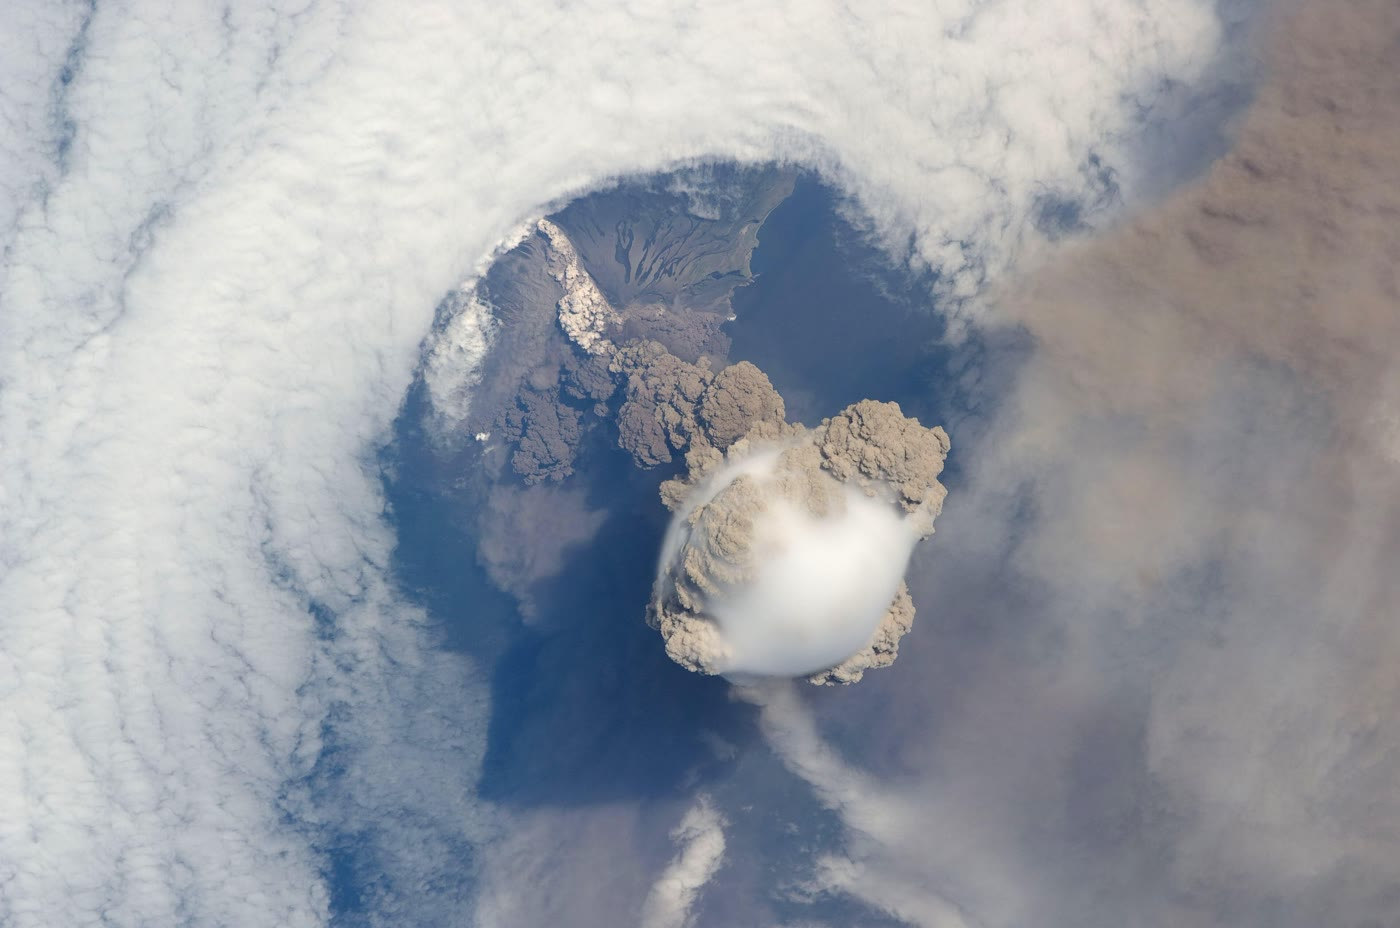
\includegraphics[width=0.66\linewidth]{images/book3/b1-sarychev-iss.jpg}
\par\smallskip{\small 萨雷切夫峰，为位于马图阿
岛上的千岛弧火山，2009 年 6 月 12 日处于喷发初期，由
国际空间站经云层中的一个空隙拍摄。灰色火山灰，很可能为火山碎屑流，自
峰顶倾泻而下，光滑的云盖（即帽状云）覆于上升的烟柱之上；
喷发产生的火山灰被探测到的距离超过
\qty{2400}{km}。照片：NASA，公有领域（维基
共享资源）。}
\label{fig:b1:active-margins:sarychev}
\end{omfigure}
% ledger: nasa:sarychev, commons:sarychev

弧下的\omterm{def:b1:layered-earth:layers}{地壳}既因缩短而增厚，也因
自下方加入的岩浆而增厚；在建于大陆之上的弧下，例如安第斯山脉之下，
它是地球上最厚的\omterm{def:b1:layered-earth:layers}{地壳}之一。

在某些弧后，上覆板块被拉开。丹·卡里格于
1971 年在板块构造框架内解释了西太平洋的这些边缘海盆地：
当板片陡倾下沉并向后回撤时，\omterm{def:b1:active-margins:active-margin}{海沟}与弧
向下沉板块一侧迁移，其后方的板块被拉伸，直至
断裂，有时在远侧留下一个已灭绝的残余弧。在上文的板块模型中，
弧后扩张速率约为 \qty{32}{mm.\text{年}^{-1}}，
位于北纬 \ang{18} 附近的马里亚纳海槽，而在汤加弧后的
劳盆地北部则超过 \qty{110}{mm.\text{年}^{-1}}。板片较浅时则相反，
它拖拽上覆板块，使其\omterm{def:b1:layered-earth:layers}{地壳}
在弧后缩短增厚，正如安第斯山脉之后那样。
% ledger: karig:marginal-basins, data:pb2002 (ridge_budget.py: Mariana 32.4, Lau 117.5 mm/yr)

\begin{inthefield}[海啸预警]
海啸预警中心只有几分钟的时间。2011 年，日本东北部海岸的首次预警
在地震后约 3 分钟发出，依据的是
短周期地震波所得的震级；对于
8 级及以上的地震，这种震级被低估，海啸高度也随之被低估。
矩震级不会饱和，但其得出约需
15 分钟：日本的宽频带地震仪已被推至量程之外。
自 2013 年起，因如此巨大地震的规模难以确定，
首次预警假定该处可能发生的最大地震，并
以“巨大”等文字描述海啸，而不给出数值，同时
预报则依据对海面本身的近海测量，来自由卫星定位的浮标，
以及布设于海底的压力计，它们能在海啸波
抵达海岸前探测到它。
% ledger: jma:warning

\smallskip
\begin{center}
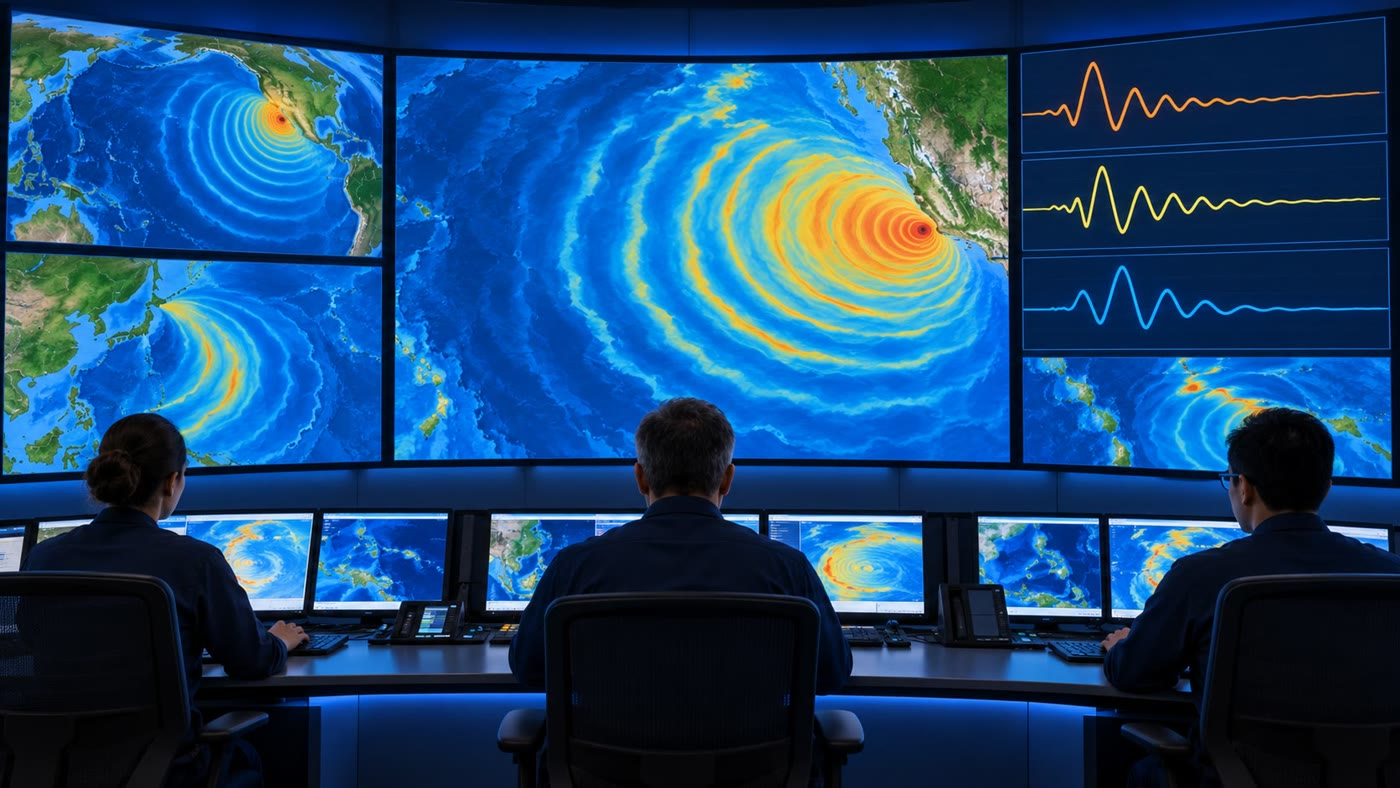
\includegraphics[width=0.7\linewidth]{images/book3/ai/b1-tsunami-centre.jpg}

{\scriptsize 海啸预警中心的值班人员，面前是
计算得出的海啸波前与海平面记录的屏幕（AI 生成插图）。}
\end{center}
\end{inthefield}

\section{练习}

\begin{exercise}[$\star$]\label{exo:b1:active-margins:1}
\omterm{def:b1:active-margins:active-margin}{海沟}位于周围洋底之下 \qty{3}{km}。(a) 若该处未被补偿，
缺失的岩石（密度为
\qty{2700}{kg.m^{-3}}）被密度为 \qty{1000}{kg.m^{-3}} 的海水取代，
该处的重力会降低多少？取布格板，其中
$G = \qty{6.674e-11}{m^3.kg^{-1}.s^{-2}}$。(b) 将结果与观测到的
千岛\omterm{def:b1:active-margins:active-margin}{海沟}上方的异常（约 \qty{-260}{\milli\gal}），
此处\omterm{def:b1:active-margins:active-margin}{海沟}位于周围洋底之下 \qty{3.5}{km}：对该深度重做计算。
(c) 为何宽度仅数十千米的\omterm{def:b1:active-margins:active-margin}{海沟}中的水给出的
结果小于板片公式，其余的亏损必须位于何处？
\end{exercise}

\begin{exercise}[$\star$]\label{exo:b1:active-margins:2}
太平洋板块以 \qty{82}{mm.\text{年}^{-1}} 的速率进入千岛\omterm{def:b1:active-margins:active-margin}{海沟}。(a) 在 1000 万年内，
有多长的板块下沉？(b) 若板片沿\omterm{def:b1:geological-maps:attitude}{倾角}为 \ang{45} 的直线路径下沉，
则其前缘此时的深度为多少？(c)
要达到 \qty{600}{km}，需要多长时间？
\end{exercise}

\begin{exercise}[$\star$]\label{exo:b1:active-margins:3}
火山位于直线形板片深度为 \qty{110}{km} 之处的上方。
计算\omterm{def:b1:geological-maps:attitude}{倾角}分别为 \ang{30}、\ang{45} 与
\ang{60} 的板片的\omterm{def:b1:active-margins:volcanic-arc}{弧沟间隙}。哪一条弧距其\omterm{def:b1:active-margins:active-margin}{海沟}最远？
\end{exercise}

\begin{exercise}[$\star$]\label{exo:b1:active-margins:4}
在本章的数字板块模型中，每年约有 \qty{2.7}{km^2} 的洋底
沿俯冲边界下沉，沿线长约
\qty{51000}{km}；同时约有 \qty{3.0}{km^2} 的洋底
\qty{67000}{km} 长的扩张脊生成。(a) 计算平均汇聚速率与
平均\omterm{def:b1:plate-kinematics:spreading-rate}{全扩张速率}，单位为 \unit{mm.\text{年}^{-1}}。(b) 在全部边界上，
模型消亡的洋底面积与生成的面积相同。其余的
新洋底去往何处？
% ledger: data:pb2002 (ridge_budget.py: 2.739 km2 over 51471 km; 3.009 km2 over 67340 km; all 3.511 vs 3.519)
\end{exercise}

\begin{exercise}[$\star\star$]\label{exo:b1:active-margins:5}
某剖面上的四次地震位于 $(x, z) = (200, 150)$、$(300, 250)$，
$(400, 330)$ 与 $(500, 430)$（单位：千米）。(a) 用最小
二乘法拟合板片直线并给出其\omterm{def:b1:geological-maps:attitude}{倾角}。(b) 该直线在何处到达地表？
(c) 与仅经过首末两次地震的直线\omterm{def:b1:geological-maps:attitude}{倾角}作比较。
\end{exercise}

\begin{exercise}[$\star\star$]\label{exo:b1:active-margins:6}
某模型板片自\omterm{def:b1:active-margins:active-margin}{海沟}起以 \ang{25} \omterm{def:b1:geological-maps:attitude}{倾角}下倾至 \qty{50}{km} 深处，
然后以 \ang{45} 倾斜。火山前缘位于板片深度为 \qty{110}{km} 之处。(a)
计算\omterm{def:b1:active-margins:volcanic-arc}{弧沟间隙}。(b) 与始终以 \ang{45} 倾斜的板片比较，
(c) 将深部段向上延伸，它到达地表之处在何处？可与
千岛直线比较：后者在\omterm{def:b1:active-margins:active-margin}{海沟}陆侧 \qty{53}{km} 处到达地表。(d)
\omterm{def:b1:geological-maps:attitude}{倾角}为 \ang{60} 的深部段会给出怎样的间隙？
\end{exercise}

\begin{exercise}[$\star\star$]\label{exo:b1:active-margins:7}
(a) 由弯曲壳层命题，弧的角半径，以及以千米计的半径
（$R = \qty{6371}{km}$），在\omterm{def:b1:geological-maps:attitude}{倾角}分别为
\ang{45}、\ang{30} 与 \ang{70} 的板片之上，弧应具有多大？(b) 哪些弧弯曲最剧烈？(c)
千岛板片\omterm{def:b1:geological-maps:attitude}{倾角}为 \ang{44.9}，千岛\omterm{def:b1:active-margins:active-margin}{海沟}拟合为
角半径为 \ang{21.9} 的圆：计算其与预测值的相对差。
\end{exercise}

\begin{exercise}[$\star\star$]\label{exo:b1:active-margins:8}
取传导率为 \qty{2.5}{W.m^{-1}.K^{-1}}，地表温度为
\qty{10}{\celsius}。(a) 计算下列两处的地表温度梯度：\omterm{def:b1:active-margins:active-margin}{弧前}之下
\omterm{def:b1:heat-budget:heat-flow}{热流}损失为 \qty{35}{mW.m^{-2}}，弧后之下\omterm{def:b1:heat-budget:heat-flow}{热流}损失
为 \qty{80}{mW.m^{-2}}。(b) 将这些梯度线性外推，估算
两者在 \qty{30}{km} 深处的温度。(c) 实测弧后\omterm{def:b1:layered-earth:discontinuity}{莫霍面}温度为 800 至
\qty{900}{\celsius}。为何线性估算偏高？
% ledger: hyndman:backarc (back-arc 70-85, Moho 800-900); the forearc value is an exercise value
\end{exercise}

\begin{exercise}[$\star\star$]\label{exo:b1:active-margins:9}
在本章的板块模型中，马里亚纳海槽在北纬 \ang{18} 附近张开，
其\omterm{def:b1:plate-kinematics:spreading-rate}{全扩张速率}约为 \qty{32}{mm.\text{年}^{-1}}。(a) 将该速率以
\unit{km.Ma^{-1}} 表示，若扩张对称，并给出半速率。
(b) 按此速率，海槽张开 \qty{100}{km} 需要多长时间？
(c) 给出两条理由，说明为何不能仅凭\omterm{def:b1:active-margins:active-margin}{弧后盆地}的
宽度与现今速率直接读出其年龄。
% ledger: data:pb2002 (ridge_budget.py: mariana_18n_mm_yr 32.4)
\end{exercise}

\begin{exercise}[$\star\star\star$]\label{exo:b1:active-margins:10}
一块厚 \qty{100}{km} 的板片，沿\omterm{def:b1:geological-maps:attitude}{倾角}为
\ang{45} 的路径以 \qty{82}{mm.\text{年}^{-1}} 下沉。取 $\kappa = \qty{e-6}{m^2.s^{-1}}$。(a) 下沉至
\qty{600}{km} 需要多长时间？(b) 在此时间内，热量按
$\sqrt{\kappa t}$ 向其内部扩散多远？(c) 热量需要多长时间才能到达其中部？(d)
试就 \qty{600}{km} 处板片的温度与
其地震活动作出结论。
\end{exercise}

\begin{exercise}[$\star\star\star$]\label{exo:b1:active-margins:11}
某个\omterm{def:b1:active-margins:accretionary}{增生楔}模型的剖面呈三角形：其表面
$\alpha = \ang{4}$ 朝\omterm{def:b1:active-margins:active-margin}{海沟}倾斜，其底面以 $\beta = \ang{6}$
向下倾斜，两者相交于其趾部；增长时两角保持不变。(a)
证明其面积为 $A = \frac12 L^2(\tan\alpha + \tan\beta)$，
宽度为 $L$，且角度足够小，使后端高度为
$L(\tan\alpha + \tan\beta)$ 时成立。(b) 厚 \qty{1}{km} 的沉积物
随板块到达，板块以 \qty{40}{mm.\text{年}^{-1}} 汇聚，沉积物全部增生：
计算 1、4 和 1000 万年后的宽度。$L$ 如何随时间增长？(c) 若
一半沉积物随板片一同俯冲，结果如何？
\end{exercise}

\begin{exercise}[$\star\star\star$]\label{exo:b1:active-margins:12}
(a) 证明最小二乘直线经过均值点
$(\bar x, \bar z)$。(b) 某目录中每个深度都偏深 \qty{10}{km}。
拟合直线的斜率与截距如何变化？(c) 所有距离
$x$ 均自一个\omterm{def:b1:active-margins:active-margin}{海沟}点量起，该点的位置偏向陆侧 \qty{20}{km}，
于是每个 $x$ 都偏小 \qty{20}{km}。斜率与
截距如何变化？(d) 这两种误差是否改变\omterm{def:b1:geological-maps:attitude}{倾角}？
\end{exercise}

\section{问题：由地震读取俯冲带}

\begin{problem}[{周末问题——由八次地震看千岛板片：
下沉速度多大，其重力与热流说明什么，
火山应位于何处}]
\label{pb:b1:active-margins:1}
% values: calc/ch14.py; the eight events are real (USGS catalogue, rounded to the km)
% from figdata/out/bachelor-1-slab_seismicity-section.dat
% ledger: data:b3-usgs-kuril, data:pb2002, data:b2-seafloor-age, syracuse:arc-depth, frank:arcs,
% data:b3-grav-kuril, parsons:plate-model, hyndman:backarc; the forearc heat flow is an exercise value
千岛板片上的八次地震，震源深度均大于 \qty{70}{km}，
沿剖面线按其距\omterm{def:b1:active-margins:active-margin}{海沟}的距离 $x$（朝向鄂霍次克海）及深度 $z$ 列出，
两者均取至千米。

\begin{center}
\small
\begin{tabular}{lcccccccc}
\hline
事件 & 1 & 2 & 3 & 4 & 5 & 6 & 7 & 8\\
$x$ (\unit{km}) & 155 & 222 & 305 & 319 & 431 & 533 & 578 & 609\\
$z$ (\unit{km}) & 96 & 169 & 245 & 272 & 389 & 489 & 518 & 573\\
震级 & 5.5 & 5.1 & 5.0 & 5.4 & 5.3 & 5.3 & 5.2 & 6.4\\
\hline
\end{tabular}
\end{center}

\medskip
\noindent\textbf{第一部分——板片线。}
\begin{enumerate}
  \item 在两轴取相同比例，画出八次地震的位置，
        深度竖直向下。
  \item 计算 $\sum x_i$、$\sum z_i$、$\sum x_i^2$、$\sum x_i z_i$ 及
        均值 $\bar x$ 与 $\bar z$。
  \item 计算 $S_{xx}$ 与 $S_{xz}$，进而求出最小二乘直线的
        斜率（精确到小数点后三位）及截距（精确到小数点后一位）。
  \item 求板片的\omterm{def:b1:geological-maps:attitude}{倾角}。
  \item 该直线在何处到达地表？这说明
        \omterm{def:b1:active-margins:active-margin}{海沟}附近板片的形状有何特征？
  \item 计算每次地震的偏差 $z_i - (a + s x_i)$。
        哪些地震离该直线最远？相距多远？
\end{enumerate}

\medskip
\noindent\textbf{第二部分——板片下沉有多快。}本节开头，
PB2002 模型给出汇聚速率为 \qty{87.4}{mm.\text{年}^{-1}}：相对于鄂霍次克板块，
太平洋板块朝\omterm{def:b1:spherical-astronomy:horizontal}{方位角} \ang{300} 方向运动。
与\omterm{def:b1:active-margins:active-margin}{海沟}垂直的剖面线朝\omterm{def:b1:spherical-astronomy:horizontal}{方位角} \ang{320.9} 方向延伸。
\begin{enumerate}[resume]
  \item 计算汇聚方向与剖面线之间的夹角，
        再求汇聚速率垂直于\omterm{def:b1:active-margins:active-margin}{海沟}的分量与
        平行于\omterm{def:b1:active-margins:active-margin}{海沟}的分量。
  \item 在 1000 万年内，有多长的板块沿\omterm{def:b1:active-margins:active-margin}{海沟}下沉？
  \item 取第 4 问中的\omterm{def:b1:geological-maps:attitude}{倾角}（取整为 \ang{45}），
        板片将其顶部某点从\omterm{def:b1:active-margins:active-margin}{海沟}带至
        该带最深地震所在处 \qty{632}{km}，需多长时间？略去
        靠近\omterm{def:b1:active-margins:active-margin}{海沟}处较缓的\omterm{def:b1:geological-maps:attitude}{倾角}。
  \item 板块在\omterm{def:b1:active-margins:active-margin}{海沟}处的年龄约为 \qty{122}{Ma}。
        现位于 \qty{632}{km} 深处的海底年龄为多少？
  \item 由 $\sqrt{\kappa t}$，取 $\kappa = \qty{e-6}{m^2.s^{-1}}$，
        在此下沉期间，热量已向板片内扩散了多远？与其
        厚度（约 \qty{100}{km}）相比较。
\end{enumerate}

\medskip
\noindent\textbf{第三部分——重力与\omterm{def:b1:heat-budget:heat-flow}{热流}。}取传导率为
\qty{2.5}{W.m^{-1}.K^{-1}}。
\begin{enumerate}[resume]
  \item \omterm{def:b1:active-margins:active-margin}{海沟}前方的老洋底约损失
        \qty{43}{mW.m^{-2}}，弧后约损失 \qty{80}{mW.m^{-2}}，\omterm{def:b1:active-margins:active-margin}{弧前}
        取 \qty{35}{mW.m^{-2}}，计算三处
        各自近地表的温度梯度。
  \item 解释为何\omterm{def:b1:active-margins:active-margin}{弧前}损失的热量
        比其前方的老洋底更少。
  \item 千岛\omterm{def:b1:active-margins:active-margin}{海沟}上方的\omterm{def:b1:isostasy-gravity:anomalies}{自由空气异常}约为
        \qty{-260}{\milli\gal}。密度为 \qty{1700}{kg.m^{-3}}
        （大于水的密度）的岩石须达多厚，布格板才能给出此亏损？
        将所得厚度与\omterm{def:b1:active-margins:active-margin}{海沟}相对周围海底的深度比较，
        后者约为 \qty{3.5}{km}。
  \item 设整个板块被下压 \qty{3.5}{km}：
        其顶部的岩石被水取代，其底部的\omterm{def:b1:layered-earth:layers}{地壳}取代了
        \omterm{def:b1:layered-earth:layers}{地幔}的位置，总之，密度为
        \qty{3300}{kg.m^{-3}} 的\omterm{def:b1:layered-earth:layers}{地幔}被水取代。计算布格板
        异常。为何真实\omterm{def:b1:active-margins:active-margin}{海沟}仅宽数十千米，
        所给出的异常却更小？
  \item \omterm{def:b1:active-margins:active-margin}{海沟}与外隆起均未处于\omterm{def:b1:isostasy-gravity:isostasy}{地壳均衡}之中，
        是什么使它们保持在均衡之外？
\end{enumerate}

\medskip
\noindent\textbf{第四部分——火山应位于何处。}用第
3 问中的直线，采用其取整后的斜率与截距。
\begin{enumerate}[resume]
  \item 该带中第一座火山距\omterm{def:b1:active-margins:active-margin}{海沟} \qty{164}{km}，
        其下方板片深度为多少？
  \item 该深度是否落在弧下观测到的
        72 至 \qty{173}{km} 范围内？它与平均值 \qty{105}{km} 相差多少？
  \item 板片深度为 \qty{100}{km} 时，距\omterm{def:b1:active-margins:active-margin}{海沟}多远？
  \item 由弯曲壳命题，千岛弧的角半径应为多少，
        以千米计的半径又为多少？
  \item 千岛\omterm{def:b1:active-margins:active-margin}{海沟}拟合一个 \ang{21.9} 的\omterm{def:b1:spherical-astronomy:spherical-triangle}{小圆}。请进行比较。
  \item \omterm{def:b1:active-margins:volcanic-arc}{火山弧}上的火山平均位于板片深度约
        \qty{105}{km} 的位置上方。板片直线在距\omterm{def:b1:active-margins:active-margin}{海沟}多远处
        达到该深度？
  \item 将此距离与观测到的 \qty{164}{km} 比较：相差多少
        千米，相差比例为多少？
  \item 取至最接近的千米数，千岛板片直线对
        位于 \qty{105}{km} 深板片上方的火山，预测的\omterm{def:b1:active-margins:volcanic-arc}{弧沟间隙}为多少？
\end{enumerate}
\end{problem}
